\documentclass[a4paper,12pt]{report}

% Pacotes necessarios
\usepackage[utf8]{inputenc}
\usepackage[brazil]{babel}
\usepackage{graphicx}
\usepackage{amsmath}
\usepackage{amsfonts}
\usepackage{amssymb}
\usepackage{geometry}
\geometry{left=3cm, right=2cm, top=3cm, bottom=2cm}
\usepackage{minted}
\usepackage{algorithm}
\usepackage{algpseudocode}
\usepackage[bookmarksdepth=subsection]{hyperref}
\usepackage{float}
\usepackage{enumitem}
\usepackage{graphicx}

\usepackage{listings}
\usepackage{xcolor}

\definecolor{codegreen}{rgb}{0,0.6,0}
\definecolor{codegray}{rgb}{0.533,0.176,0.376}
\definecolor{codepurple}{rgb}{0.58,0,0.82}
\definecolor{backcolour}{rgb}{0.95,0.95,0.92}
\definecolor{new_blue}{rgb}{0, 0.7, 2}
\definecolor{new_red}{rgb}{0.70, 0.047, 0}
\definecolor{new_pink}{rgb}{2.55, 0 , 2.03}



\lstdefinestyle{octstyle}{
    language=Octave,
    basicstyle=\ttfamily\small\color{new_blue},
    keywordstyle=\color{blue},
    stringstyle=\color{new_red},
    commentstyle=\color{new_pink}\itshape,
    numbers=left,
    numberstyle=\tiny\color{new_pink},
    breaklines=true,
    showstringspaces=false,
    frame = shadowbox,
}
\lstdefinestyle{output}{
    language=Bash,
    basicstyle=\ttfamily\small\color{blue},
    keywordstyle=\color{blue},
    stringstyle=\color{codegreen},
    commentstyle=\color{codegreen}\itshape,
    numbers=left,
    numberstyle=\tiny\color{blue},
    breaklines=true,
    showstringspaces=false,
    frame = shadowbox,
}


% Configuracao de cabecalhos e rodapes
\usepackage{fancyhdr}
\pagestyle{fancy}
\fancyhf{}
\fancyhead[L]{Engenharia de Sistemas}
\fancyhead[R]{Documentação Drone Resgate }
\fancyfoot[C]{\thepage}

% Configuracao para referencias
\usepackage{cite}

% Documento
\begin{document}

% Capa
\begin{titlepage}
    \begin{center}
       
        {\Large Universidade Federal de Santa Catarina}\\[1.5cm]
        {\Large Engenharia de sistemas}\\[3cm]
        
        {\LARGE\textbf{Documentação Drone Resgate}}\\[2cm]
        
        \textbf{Eduardo Koscianski,\\
        Marcos Antonio\\
        Willians\\
        Giuliano}\\[4cm]
        \includegraphics[width=0.30\linewidth]{images/ufsc.png}\\     
        \vfill
        Joinville - SC\\
        2025
    \end{center}
\end{titlepage}

% Folha de Rosto
\begin{titlepage}
    \begin{center}
      {\Large Universidade Federal de Santa Catarina}\\[1.5cm]
        {\Large Engenharia Mecatronica \&  Engenharia Aeroespacial}\\[3cm]
        
        {\LARGE\textbf{Documentação drone Resgate}}\\[2cm]
        
        \textbf{Marcos Antonio Tome Oliveira}\\[4cm]
      \includegraphics[width=0.50\linewidth]{images/drone.jpeg}\\ 
      
        
        \vfill
        Joinville - SC\\
        2024
    \end{center}
\end{titlepage}

% Sumario
\tableofcontents
\listoffigures
%\lstlistoflistings
\newpage
\section{Definições}
\textbf{Como uma equipe, discuta, converse e escreva uma definição para os itens a seguir. Essas
definições devem ser originais. Isso significa que você não deve procurá-las em um livro ou na
Internet, mas criá-las você mesmo com base em sua experiência anterior, no que aprendeu na aula
até agora e nas discussões entre a equipe. Se não for possível chegar a uma definição específica,
você deve dizer isso e por que, em seguida fornecer a(s) definição(ões) alternativa(s). O processo a ser seguido para tentar chegar a um consenso fica a seu critério.}
\begin{itemize}
    \item \textbf{Sistema}
Um sistema é um conjunto de partes que trabalham juntas para alcançar um objetivo. Pode ser um software, uma máquina, um processo de negócios ou até mesmo uma equipe – o importante é que os componentes interajam de forma coordenada para que o todo funcione como esperado. 
\item \textbf{Engenharia}
Engenharia é a aplicação prática de conhecimentos científicos e técnicos para criar, melhorar ou resolver problemas em estruturas, produtos ou processos. Seja desenvolvendo um novo dispositivo, otimizando uma operação ou garantindo que algo seja seguro e eficiente, a engenharia transforma ideias em realidade.  
\item \textbf{Engenharia de Sistemas}
É a disciplina que organiza e integra diferentes partes de um projeto complexo, garantindo que tudo funcione em harmonia. Enquanto outros engenheiros focam em áreas específicas (como eletrônica ou software), a engenharia de sistemas cuida da visão geral, dos requisitos até a entrega, para que o resultado final atenda às necessidades do usuário e do negócio.  
\item 
\textbf{Parte Interessada (Stakeholder)}  
São todas as pessoas ou grupos impactados por um projeto, seja direta ou indiretamente. Isso inclui clientes, usuários, gerentes, fornecedores e até reguladores. Entender suas expectativas é essencial para o sucesso, pois são eles que vão avaliar se o resultado atendeu ao que era esperado.  
\item \textbf{Marco (Milestone)}
Um marco é um ponto-chave no cronograma que marca a conclusão de uma etapa importante. Não é apenas uma data, mas um momento para revisar o progresso e ajustar rumos.
\item \textbf{Necessidade}
A necessidade é algo essencial - seja físico, emocional ou funcional.
É o problema ou oportunidade que justifica o projeto. Identificar corretamente as necessidades evita soluções bem construídas, mas que não resolvem o que realmente importa
\end{itemize}

\section{Análise das partes interessadas}
\subsection*{}
\textbf{Você também pode procurar outras fontes de dados (inclusive na Internet) para ler sobre a história de algum projeto semelhante e qualquer outra informação relevante sobre este ou outros projetos semelhantes.}

\subsection*{}
\textbf{Identifique cuidadosamente as partes interessadas envolvidas no projeto. Forneça uma breve descrição de cada parte interessada em poucas frases. Concentre-se em suas funções, necessidades e objetivos.}

\begin{itemize}
    \item Órgãos Governamentais
São instituições públicas nacionais, estaduais ou municipais interessadas em adquirir tecnologias que aprimorem a resposta a desastres naturais. Seu objetivo é garantir soluções eficientes, seguras e de custo viável para operações de resgate em larga escala, como em enchentes. Esses órgãos também são responsáveis por aprovar, regulamentar e financiar o uso de tecnologias no contexto de defesa civil.
\item  Corpo de Bombeiros
Principal instituição responsável por ações de busca e salvamento em situações de emergência. Necessitam de uma solução robusta, confiável e fácil de operar em campo, que auxilie na localização de vítimas e mapeamento de áreas afetadas, reduzindo riscos aos seus agentes e otimizando os esforços de resgate.

\item  - Equipe de Treinamento e Operação
Profissionais técnicos responsáveis por capacitar os operadores do drone. Precisam conhecer tanto os aspectos específicos da aeronave (como autonomia, sensores e rotas) quanto os requisitos operacionais em campo. Suas necessidades envolvem documentação clara, interface de controle intuitiva e acesso a suporte técnico.

\item   Vítimas e Comunidades Afetadas
Embora não operem diretamente o sistema, são o público-alvo da missão do drone. As necessidades dessas pessoas devem influenciar as decisões do projeto: rapidez no resgate, precisão na localização, e confiabilidade da missã

\item  Equipe de Desenvolvimento (Engenheiros e Programadores)
São os responsáveis por projetar e implementar o drone. Precisam de requisitos bem definidos, acesso a recursos (hardware e software) e feedback constante das demais partes interessadas para garantir que o produto atenda às expectativas.

\item  ONGs e Instituições Humanitárias
Muitas vezes estão envolvidas em apoio a desastres e podem ser parceiras no uso do drone em áreas de difícil acesso ou em regiões com pouco suporte governamental.
\item  Investidores - Atores interessados em financiar o desenvolvimento e a implementação da tecnologia, seja por retorno social, alinhamento com causas humanitárias ou perspectivas de investimento sustentável. Buscam transparência, viabilidade e impacto real na solução proposta.
\end{itemize}

\subsection*{}
\textbf{Crie uma tabela em que, para cada parte interessada identificada acima, você liste seus inputs e outputs em termos de fluxos de valor. Para encontrar os inputs, pergunte o que cada um deles precisa receber de outros participantes para cumprir sua função. Exemplos de fluxos de valor são informações, dinheiro, aprovações, bens físicos, serviços etc. ..... Seja o mais específico possível. Os resultados são coisas fornecidas por um participante para um ou mais outros participantes. Um exemplo dessa tabela é mostrado na aula anterior.}

\begin{table}[H]
\centering
\caption{Fluxos de Valor entre Partes Interessadas}
\resizebox{\textwidth}{!}{
\begin{tabular}{|p{4cm}|p{4cm}|c|p{5cm}|p{5cm}|}
\hline
\textbf{Stakeholder A} & \textbf{Stakeholder B} & \textbf{Pontuação de Influência Mútua} & \textbf{Inputs (de A para B)} & \textbf{Outputs (de B para A)} \\
\hline
Órgãos Governamentais & Corpo de Bombeiros & 0{,}89 & Legislação, financiamento, autorização & Relatórios, pareceres técnicos, laudos \\
\hline
Corpo de Bombeiros & Investidores & 0{,}50 & Relatórios de vistoria, certificações & Financiamento, suporte a infraestrutura \\
\hline
Corpo de Bombeiros & Treinadores & 0{,}40 & Necessidades de formação, exigências técnicas & Capacitação, programas de treinamento \\
\hline
Projeto & Governo Local & 0{,}59 & Relatórios de progresso, propostas & Licenciamento, apoio político \\
\hline
Empresa & Fornecedores & 0{,}45 & Pagamentos, contratos, especificações & Entrega de materiais, serviços \\
\hline
Projeto & Empresa & 0{,}65 & Especificações técnicas, desenhos CAD, requisitos de engenharia & Protótipos físicos, produção em série, feedback técnico sobre viabilidade \\
\hline
\end{tabular}}
\end{table}

\subsection*{}
\textbf{Crie duas versões de um mapa de rede das partes interessadas. Primeiro, crie um modelo clássico de "hub-and-spoke" em que sua equipe seja a organização central. Isso significa que apenas as entradas/saídas que envolvem sua equipe diretamente da tabela acima serão exibidas. Em segundo lugar, crie um mapa completo da Rede de Valor das Partes Interessadas (SVN) que inclua todas as entradas/saídas da tabela e provavelmente também incluirá relações indiretas que não envolvam a sua equipe. Use setas coloridas para criar o mapa SVN.\\
Comente sobre as percepções que você conseguiu obter com essa análise das partes interessadas do projeto, se houver.}
\begin{figure}[h!]
    \centering
    \includegraphics[width=0.80\linewidth]{hub_spoke.png}
    \caption{hub-spoke}
    \label{hub-spoke}
\end{figure}
\begin{figure}[h!]
    \centering
    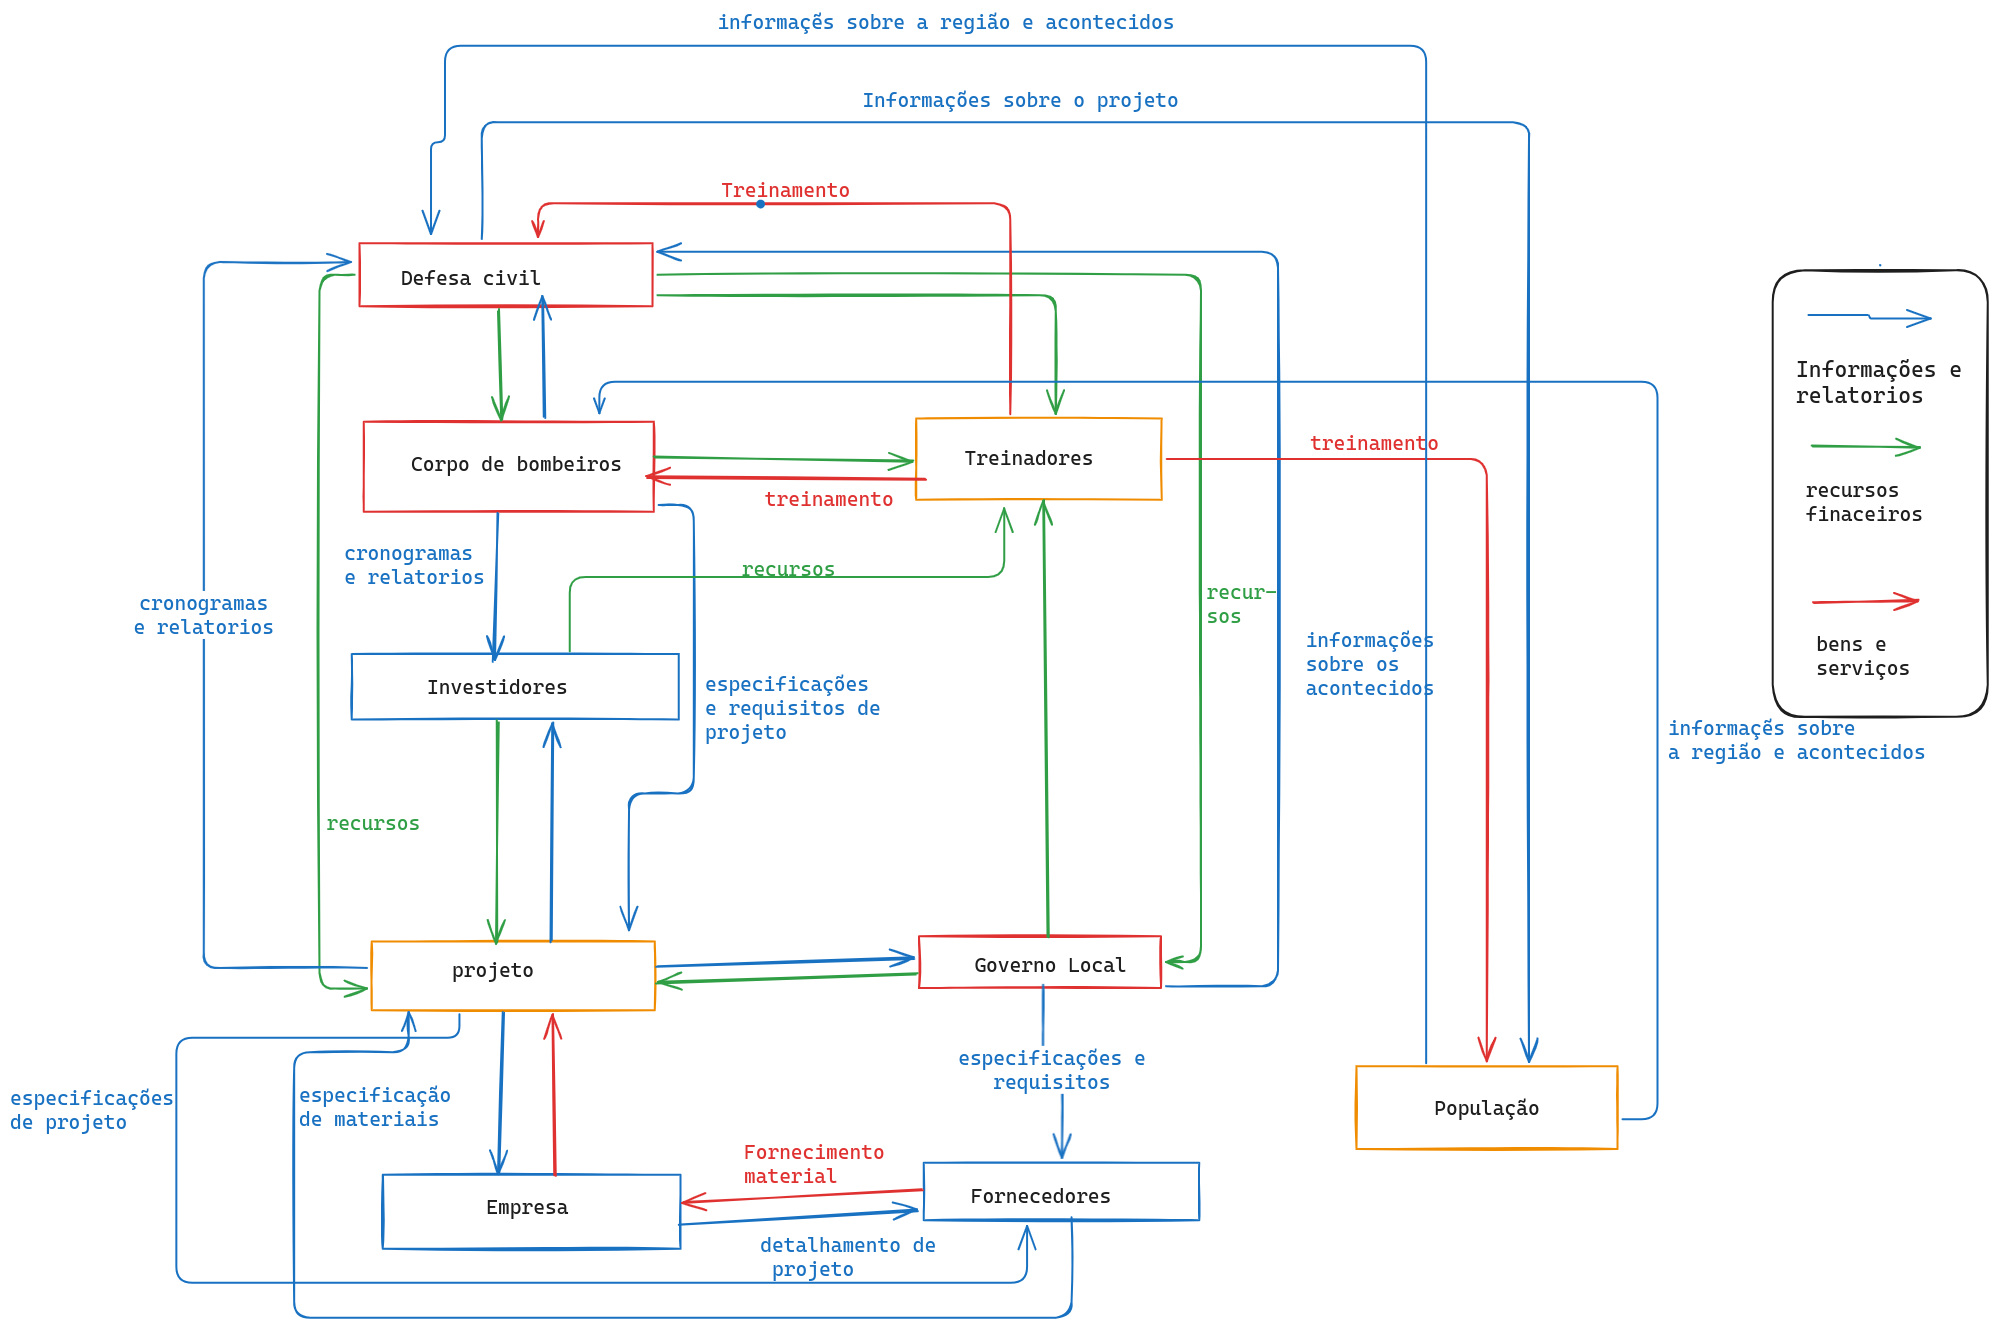
\includegraphics[width=0.75\linewidth]{svn.png}
    \caption{svn}
    \label{svn}
\end{figure}

\begin{itemize}
    \item - **Corpo de Bombeiros** é um elo central, recebendo inputs regulatórios e influenciando vários outros (investidores e treinadores).
    \item  - **Investidores** dependem diretamente da avaliação técnica do Corpo de Bombeiros, o que mostra a **importância da segurança para a continuidade do financiamento**.    

    \item  - **Órgãos Governamentais** têm alta influência, mas poucos retornos diretos — sua atuação é mais normativa.
   \item  - **Fornecedores** são mais reativos no sistema: recebem e executam, com pouca influência estratégica.
   \item - O **projeto (sua equipe)** está no coração da interação com governo local e bombeiros, e indiretamente afeta todo o ecossistema.
\end{itemize}



    

    

    






\end{document}